\documentclass{aa}
\usepackage[varg]{txfonts}
\usepackage{nicefrac}
\usepackage{caption}
\usepackage{listings}
\usepackage{xcolor}
\usepackage{siunitx}
\usepackage{tikz}
\usepackage{hyperref}

\definecolor{paper}{RGB}{235,213,179}
\definecolor{orange}{RGB}{255,79,0}

\hypersetup{colorlinks,
            linkcolor=blue,
            citecolor=blue,
            urlcolor=blue}

\begin{document}

\lstset{language=Python,
        xleftmargin=2em,
        backgroundcolor=\color{paper},
        numbers=left,
        numbersep=5pt,
        numberstyle=\tiny,
        rulecolor=\color{black},
        keywordstyle=\color{orange},
        basicstyle=\footnotesize,
        breaklines=true,
        breakatwhitespace=true,
        escapeinside=||}

\let\origthelstnumber\thelstnumber
\makeatletter
\newcommand*\Suppressnumber{%
  \lst@AddToHook{OnNewLine}{%
    \let\thelstnumber\relax%
     \advance\c@lstnumber-\@ne\relax%
    }%
}

\newcommand*\Reactivatenumber[1]{%
  \setcounter{lstnumber}{\numexpr#1-1\relax}
  \lst@AddToHook{OnNewLine}{%
   \let\thelstnumber\origthelstnumber%
   \refstepcounter{lstnumber}
  }%
}

\title{Assignment 3}

\subtitle{Direct Simulation Monte Carlo and parallelization.}

\author{David Hernandez\inst{1}}


\institute{Universität Wien, Institut für Astrophysik, Türkenschanzstrasse
17, 1180 Wien, Austria}

\date{Deadline: December 12\textsuperscript{th}, 2020 / Submitted: December
5\textsuperscript{th}, 2020}

\abstract{Two Python scripts were written in order to compute the constant Pi (\(\pi\)) using
the Direct Simulation Monte Carlo (DSMC) method. To achieve this goal a python class was
implemented and used in both codes. The second script does the exact same calculations, only
multiprocessing was introduced in order to speed up the total runtime of the program. The
program was tested with a maximum number of \num{10000} particles were introduced to determine
\(\pi\). The computations were done for all numbers of particles from zero up to the maximum
number. The results, the residuals and the simulation domain were displayed graphically to see
if the simulation converges. The median of all results was accurate within \num{+-0.02} of the
true value of pi. Multiprocessing sped up the computations by a factor of \num{2.13} when using
8 cores on an Intel i7-6700HQ Processor clocked at \SI{3.5}{\giga\hertz}.}

\keywords{Numerical methods -- Direct Simulation Monte Carlo -- Pi -- Multiprocessing}
\maketitle

\section{Introduction}%
\label{sec:introduction}

When doing complex computations it may sometimes be the case, that the actual
calculations take too long or are too complicated to be easily solved. Then we can resort to
statistics in order to approximate the true solution, hence either reducing the time needed for
the computations or simplifying the problem at hand.

To demonstrate the method, the constant \(\pi\) shall be determined. In general we can compute
\(\pi\) if we know the area of a circle with radius \(r\) as follows.
\begin{equation}
    \label{eqn:circle_area}
    \pi = A_\mathrm{circ} / r^2
\end{equation}
Unfortunately it is not trivial to measure the are of a circle, therefore we shall consider a
square with side length \(2r\), enclosing the circle (Figure \ref{fig:domain}), and compute its
area.
\begin{equation}
    \label{eqn:area_square}
    A_\mathrm{squa} = 4r^2
\end{equation}
No by rearranging for \(r^2\) and substituting into Equation \ref{eqn:circle_area} we get the
following expression for computing \(\pi\).
\begin{equation}
    \label{eqn:pi}
    \pi = 4 \frac{A_\mathrm{circ}}{A_\mathrm{squa}}
\end{equation}
But as mentioned above we do not know the area of the circle, but what we can do is estimate
the fraction of the two areas by randomly scattering particles over the whole domain of the
square and circle.
\begin{figure}[htbp]
    \centering
    \captionsetup{width = 0.9 \linewidth}
        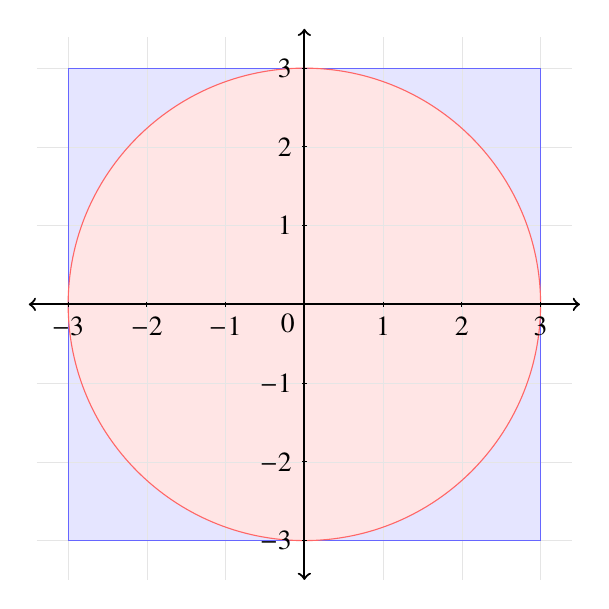
\begin{tikzpicture}
            \fill[fill=blue!10] (-3,-3) -- (3,-3) -- (3,3) -- (-3,3) -- cycle;
            \fill[fill=red!10] (0,0) circle (3);
            \draw[step=1, gray!20, very thin] (-3.4,-3.5) grid (3.4,3.4);
            \draw[blue!60] (-3,-3) rectangle (3,3);
            \draw[red!60] (0,0) circle (3);
            \draw[thick, <->] (0,3.5) -- (0,-3.5);
            \draw[thick, <->] (-3.5,0) -- (3.5,0);
            \foreach \x in {-3, -2, -1, 1, 2, 3}
                \draw (\x, 1pt) -- (\x, -1pt) node[anchor=north] {\(\x\)};
            \foreach \y in {3, 2, 1, -1, -2, -3}
                \draw (1pt, \y) -- (-1pt, \y) node[anchor=east] {\(\y\)};
            \draw node[anchor=north east] {0};
        \end{tikzpicture}
    \caption{The whole simulation domain with the circle in it. In this case \(r\) equals three
    but in general the value of \(r\) is independent and can be any real value. For instance in
    the code a radius of 500 is used.}
    \label{fig:domain}
\end{figure}
If we trust that the scattering process is truly random and not influenced or biased in any
way, the fraction of particles inside the circle (\(n_\mathrm{inside}\)) and the total number
of particles (\(n_\mathrm{total}\)) in the square domain should equal to the fraction of these
two areas:
\begin{equation}
    \label{eqn:fractions}
    \frac{n_\mathrm{inside}}{n_\mathrm{total}} \overset{!}{=}
    \frac{A_\mathrm{circ}}{A_\mathrm{squa}}
\end{equation}
And therefor we can approximate \(\pi\) as shown below, if a sufficient number of particles is
used in the simulation. In principle, if we use an infinite number of particles Equation
\ref{eqn:approximation} will yield the exact result. However that is exactly what we get if we
integrate the areas ourselves, which could be considered as too much of a hassle and therefor
we resort to the DSMC method.
\begin{equation}
    \label{eqn:approximation}
    \pi \approx 4 \frac{n_\mathrm{inside}}{n_\mathrm{total}}
\end{equation}

\section{Implementation}%
\label{sec:implementation}

Two python scrips were written in order do the DSMC computation and acquire the approximate
value of \(pi\). Execution of the scripts shall be solely via the command line interface of a
PC. Any user input is passed to the program by command line arguments. Examples are shown
below.
\begin{lstlisting}[language=bash, numbers=none]
$ ./pi.py <n_particle_max>
$ ./multipi.py <n_particle_max> <n_cpu>
\end{lstlisting}

\subsection{Task 1}%
\label{sub:task_1}
For the DSMC computation a class \verb+MyPi+ was written. This method has two methods and six
public attributes. The general architecture of the class depends on the simulation domain and
the mask. Once they are set up, a number of particles is distributed randomly over the entire
domain. To count the number of particles in within the circle a boolean circular mask is
applied to the simulation domain. Finally the result for the launched number of particles is
computed and returned.

Line numbers in the following code listings correspond to the line numbers in the \verb+pi.py+
script.

\paragraph{Methods:}
\begin{itemize}
    \item \verb+__init__(size)+: This is the class constructor. When a new \verb+MyPi+ object
        is created, it sets up the simulation domain and the mask. Since the array indices are
        of integer value, the entire domain is discretised.Therefor the size of the domain has
        to be large enough in order to get decent results. In this script a domain size of
        \(1001 \times 1001\) is used. Additionally, if the size is even, a one is added to make
        it odd. This slightly simplifies computations done on the domain.
\begin{lstlisting}[firstnumber=104]
if (size % 2) == 0:
    warnings.warn('Domain size is even, Adding 1 to make odd!',
                  UserWarning)
    size += 1
self.size = size
\end{lstlisting}
        Then two arrays defined, one with datatype \verb+int+ and one with datatype
        \verb+bool+.
\begin{lstlisting}[firstnumber=104]
self.domain = np.zeros((size, size), dtype=int)
self.mask = np.zeros((size,size), dtape=bool)
\end{lstlisting}
        Then the center of the mask is determined and all positions within the circle are set
        to true. This was done by computing the distance of each position from the center where
        the indices are treated as the coordinates of the position in the domain. 
\begin{lstlisting}[firstnumber=117]
__dom_pos = np.ogrid[0:self.size, 0:self.size]
__cen_dist = np.sqrt(  (__dom_pos[0] - __center[0])**2
                     + (__dom_pos[1] - __center[1])**2)
self.mask[__cen_dist <= __radius] = True
\end{lstlisting}
    \item \verb+launch_particles(n)+: Here \(n\) particles are randomly distributed to the
        simulation domain. If \(n\) is zero, the \verb+no_particles+ flag is set to
        \verb+True+. To get the random values \verb+numpy.randint()+ was used. Two arrays with
        \(n\) random integers between zero and the domain size are created. One for the x
        coordinate and one for the y coordinate. Different seeds are used for the two sets. 
        \begin{lstlisting}[firstnumber=151]
seed()
__x = randint(0, self.size, n)
seed()
__y = randint(0, self.size, n)
        \end{lstlisting}
        The two sets are then stacked along axis 1, so that every line in the new 2D array
        holds the x and y coordinates of the particle in the domain.
        In order to determinate duplicates, a new array with the unique particle coordinates is
        created along with an array holding the number of occurrences of each particles. Then
        the unique x and y components are stored to two individual array. Finally the particles
        are distributed to the domain.
        \begin{lstlisting}[firstnumber=176]
self.domain[self.x, self.y] += __counts
        \end{lstlisting}
        Additionally the \verb+no_particles+ flag is set to \verb+True+ or \verb+False+ weather
        the number of particles is zero or not.
    \item \verb+compute()+: Get the approximation for \(\pi\). This step is rather simple, once
        the total sum of the particles is determined and once the sum of particles in the
        circle finally \(\pi\) is computed according to Equation \ref{eqn:approximation}.
        \begin{lstlisting}[firstnumber=205]
__sum2 = np.sum(self.domain)|\Suppressnumber|
[...]|\Reactivatenumber{209}|
__sum2 = np.sum(self.domain[self.mask])|\Suppressnumber|
[...]|\Reactivatenumber{213}|
return (__sum1 / __sum2) * 4
        \end{lstlisting}
\end{itemize}

\paragraph{Attributes:}
\begin{itemize}
    \item \verb+size+ : scalar\\
        The size of the simulation domain.
    \item \verb+domain+ : 2D \verb+numpy.array+\\
        The simulation domain is a two dimensional square of user defined size. The size is
        given when a new \verb+MyPi+ object is created and the constructor is called.
    \item \verb+mask+ : 2D \verb+numpy.array+\\
        A circular boolean mask where the circles radius equals to half the size of the domain.
        \(r = size / 2\)
    \item \verb+x+ : 1D \verb+numpy.array+\\
        The x component of the launched particles.
    \item \verb+y+ : 1D \verb+numpy.array+\\
        The y component of the launched particles.
    \item \verb+no_particles+ : scalar\\
        A boolean flag to determine if any particles are created.
\end{itemize}

\paragraph{Main subroutine:}
This is the part of the script where all the parts come together. First a new \verb+MyPi+
object is created and the maximum number of particles is read from the command line arguments.
\begin{lstlisting}[firstnumber=236]
pi = MyPi(1001)
n_max = int(sys.argv[1])
\end{lstlisting}
The computation is done ten times in order to determine if there is a different result each
time the calculations are done. Given the random nature of the DSMC method, this is expected.
The approximation of \(pi\) is done for each number of particles in the total number of
particles specified by the user when the code is executed. The result that is retrieved for
each number of particles is stored to an array.
\begin{lstlisting}[firstnumber=257]
for j, n in enumerate(range(n_max)):|\Suppressnumber|
    [...]|\Reactivatenumber{268}|
    pi.launch_particles(n)
    results[j] = pi.compute()
\end{lstlisting}
Finally the estimated values for pi and the residuals from each of the ten runs are the median
of the results produced in one run. The results from the last run are then used to create the
plots that show convergence. To plot the domain, 1000 particles are launched, so that the
random distribution of particles can be shown.
\begin{lstlisting}[firstnumber=290]
pi.launch_particles(1000)
\end{lstlisting}

\subsection{Task 2}%
\label{sub:task_2}

For the second task the exact same thing was computed as in task one. However this time
parallel computing is introduced. When parallelsing code one first needs to make sure that part
that shall be processed concurrently is independent from all other instances of the
parallelization. Considering an iterable task that depends on the result of a previous
iteration, simultaneously running multiple iterations can lead to problems as some results my
not have been produced yet, but are depended on. Take for instance an operation that computes
the following:
\begin{equation}
    \label{eqn:previous_dependence}
    y_{n} = y_{n-2} + y_{n-1}
\end{equation}
Where \(y_{n-1}\) and \(y_{n-2}\) are the results from previous iterations, then \(y_n\) can
only be determined when \(y_{n-1}\) and \(y_{n-2}\) have been computed already. Therefor, it is
impossible to do calculate the following at the same time since some results are not available
by the time the parallel execution was issued.
\begin{eqnarray}
    y_4 = y_2 + y_3\\
    y_5 = y_3 + y_4\\
    y_6 = y_4 + y_5
\end{eqnarray}

Line numbers in the following code listings correspond to the line numbers in the
\verb+multipi.py+ script. This script uses the same \verb+MyPi+ class that is described in
detail in Section \ref{sub:task_1}. Therefore only the main subroutine and the \verb+get_pi()+
wrapper function will be discussed here.

\paragraph{Wrapper function:} In order utilize multiprocessing for this code, all operations
that are done in one iteration, must be callable in a function, as is shown in the pseudo code
below:
\begin{lstlisting}[numbers=none]
for each iteration:
    operations_wrapper(args)
\end{lstlisting}
For the case at hand, the wrapper is very simple and takes only one argument, the number of
particles that are used in the current iteration. Within the wrapper a new \verb+MyPi+ object
is created and the number of particles passed to the wrapper are launched. Then the result is
computed and the \verb+MyPi+ object is deleted in order to preserve memory and finally the
result is returned.
\begin{lstlisting}[firstnumber=210]
def get_pi(particles):|\Suppressnumber|
    [...]|\Reactivatenumber{212}|
    pi = MyPi(1001)
    pi.launch_particles(particles)
    result = pi.compute()
    del pi
    return results
\end{lstlisting}

\paragraph{Main subroutine:} The multiprocessing version of the script comes with three modes
of operation.
\begin{description}
    \item[Normal:] Runs the code with the specified amount of of CPU cores, physical and/or
        logical. Command line arguments ranging from one to the maximum number of cores
        available on the machine.
    \item[Auto:] Runs the code with the maximum number of available cores, physical and/or
        logical. Command line arguments \(0\) or any number greater than the available cores on
        the machine.
    \item[Benchmark] Runs the code in benchmark mode. The script is run multiple times, each
        time with an increased number of CPU cores to assess the performance increase. This
        mode is activated by giving any negative number as command line argument.
\end{description}


\end{document}
